Chapter \ref{ch:evolution} described the various legal issues surrounding the publishing of research outputs in general and datasets in particular and hinted that repositories can help alleviate these issues by providing technological solutions that can either implement compliance or help users take informed decisions on legal aspects.

In recent years, the rise of \emph{blockchain} technologies such as Bitcoin\footnote{\url{https://bitcoin.org/}} or Ethereum\footnote{\url{https://ethereum.org/}}  has been examined as a potential mean of solving some of these issues, the movement in this direction being fuelled, in part, by the increase in interest due to usage in the financial domain (e.g., Bitcoin). At a very high level, the blockchain allows recording data and verifying its authenticity without the need for a central authority. In the most popular implementations, each participant in a blockchain holds a copy of the whole record set and each record is linked to a previous one by a cryptographic value, distilled using the records' content; thus, even the most trivial change would propagate across the whole chain, signalling the modification. The basic idea behind blockchains can prove useful in areas where authenticity, provenance, and anonymization are important, research being one of them. In \cite{dsbc} the authors have identified a number of ways in which blockchains could be implemented across the scholarly workflow, such as:

\begin{itemize}
    \item Digital rights management: a blockchain system can easily record ownership and ensure that future usage of data respects and attributes  ownership along with any associated stipulations. This could prove useful also in terms of counting citations and understanding how outputs are further reused.
    \item Hypothesis registration: allow researchers to signal a discovery, proof, or new dataset while providing evidence of ownership in any future instance.
    \item Study pre-registration: while becoming a common practice, it can be difficult to ensure that these plans are not modified while the experiments are ongoing, in order to mask potential discrepancies with the actual results; a blockchain systems could easily detect such a change.
    \item Data anonymisation and provenance: this can prove to be of utmost importance for medical and pharmacological research, where, on one hand, stringent requirements on patient privacy and data anonymisation\footnote{Refer to Section \ref{subsec:legal}} are in place, and, on the other hand, the origin of the data should be verifiable. The use of cryptographic controls and the distributed architecture of blockchain systems can help with these challenges.
\end{itemize}

The first point above presents interest, as licencing and distribution is most often closely linked to the perceptions researchers have on sharing outputs. Various studies \cite{federer,kim} have identified \emph{perceived risks} in data sharing activities, largely due to the conditioning of academic success on publication volume and impact. A survey among Wellcome Trust awardees showed that \emph{``the main barriers to data sharing are  the fear for misuse and misinterpretation of data, the fear to lose publication opportunities [\ldots]''} \cite{wellcome}. Another study on articles published in Science between 2011 and 2012 found out that 11\% of the authors refuse to share data if the requester does not provide information on how the material will be further used\cite{stodden}.

A particular blockchain technology, \emph{smart contracts} can approach these issues from a technological angle. The remaining of the chapter proposes a solution to research output licencing that uses smart contracts and blockchains to record dissemination and reuse actions; in the next section an overview of these technologies is included.

\newpage

\section{Blockchain technologies}
\label{sec:blockchain}

A blockchain is a continuously growing list of records linked using cryptographically calculated values. Each block records a cryptographic \emph{hash} value of the previous block, a timestamp, and data about one or multiple \emph{transactions} (algorithmic operations with one or more inputs and one or more outputs); such a list of transactions is called a \emph{ledger}. The transactions are encoded into a Merkle tree (or a hash tree), in which each leaf node is labelled with the cryptographic hash of a data block and every non-leaf node is labelled with the hash of the labels of its children (see Fig. \ref{fig:merkle} for an example). Most Merkle tree implementations are binary\footnote{This is not a strict requirement.} and thus verifying that a certain leaf is part of a given tree requires logarithmic time. Usually, cryptographic hash functions, such as \gls{sha2}\cite{sha2} are employed, for stronger security guarantees.

\begin{figure}[thpb]
  \centering
  % fbox will add a border around the figure
  \fbox{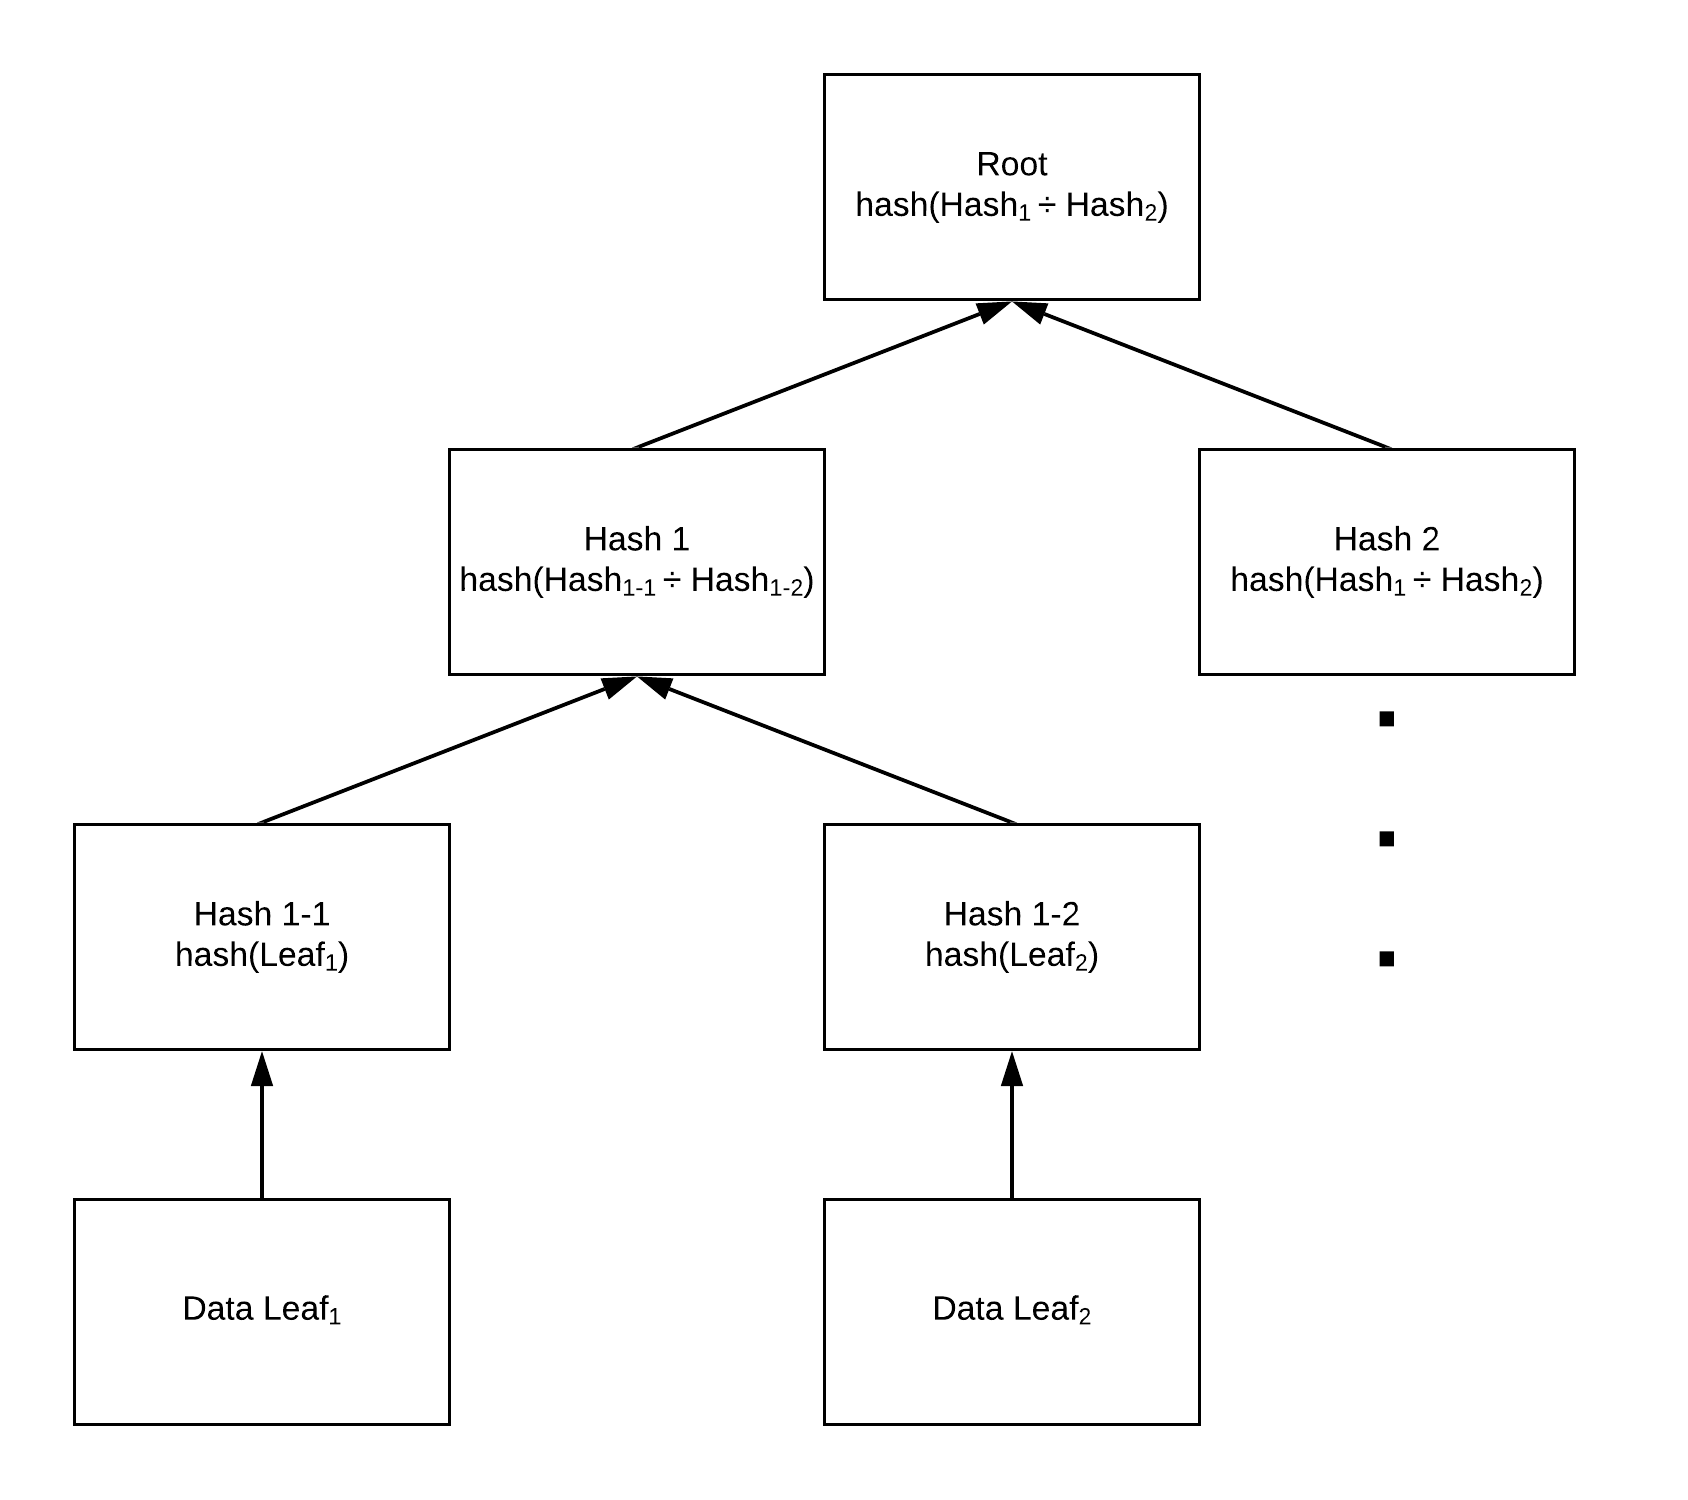
\includegraphics[scale=0.7]{figures/merkle.png}}
  \caption{An example of a binary Merkle (hash) tree. The $\div$ operator denotes a concatenation of hashes.}
  \label{fig:merkle}
\end{figure}

In a blockchain system blocks are continuously created, generating a verification chain that can be traversed up to the original \emph{genesis} block. An important aspect of these systems relates to the time required to create a block or, to be more precise, the time until each new block becomes verifiable.

It can be noted here that starting from a given block, two new blocks could be created at the same time, generating a conflict. In blockchain systems implementing currencies or other financial mechanisms this could lead to so-called \emph{double spend attacks}\footnote{For example, two simultaneous transactions that require a single value token to be extracted from an account holding a single token.}. This issue is solved by implementing algorithms that establish hierarchies among concurrent transactions, which would discard transactions leading to inconsistencies.

Most blockchain systems are implemented as a peer-to-peer network, in which each node stores a full copy of the blockchain, thus removing the requirement for a central authority that needs to verify all transaction data; practically, such systems implement a distributed database in which consensus is achieved via the proof for validating the sequence of blocks; proofs are exchanged using ad-hoc messages.

One of the more popular use-cases for blockchain relates to the implementation of cryptocurrencies, which differentiate themselves from traditional currencies by being decentralised, requiring no central entity (bank or government) for controlling the market flow. Bitcoin is such a currency, which is implemented as a public ledger in which transactions between its users are recorded; for each transaction, information such as \emph{``Alice sent Bob X bitcoins''} is broadcast to all participating peers.

Ethereum is another crptoccurency that evolved into an open platform for building decentralised applications on top of blockchains; it defines a number of protocols for running arbitrarily complex algorithms on the network. Such code is ran on \glspl{evm} which are stored on each node participating in the network; each issued instruction is ran on every node. A valid state transition on \glspl{evm} is one which comes through a transaction\cite{gavin}. Ethereum also implements its own value token, called \emph{ether}, but the way in which this is used depends on the application being implemented. One purpose of the value token is to provide a representation of the physical resources required for participating in the network (e.g., electrical power), and, for example, most commonly each operation executed on the \glspl{evm} carries an inherent cost, denoted as \emph{gas}\cite{gavin}, which is directly connected to the block time previously mentioned.

Smart contracts are a protocol which allows to digitally facilitate, verify, or enforce the negotiation and performance of a contract. Initially introduced in 1996-1997\cite{szabo}, they came back into the spotlight along with the other blockchain technologies, as a mean of verifying various types of transactions. Smart contracts aim at reducing or even removing the need of trusted third parties (e.g., arbitrators or notaries) which are mandatory in the execution of traditional contracts, while also implementing mechanism for preventing frauds and malicious or accidental exceptions.

In \cite{ethpap} the authors point out that Bitcoin is a weaker version of the smart contracts concept introduced in \cite{szabo}, due to, for example the lack of Turing-completeness or multi-step contracts. The authors argue that these limitations would prevent the Bitcoin implementation from encoding any contract instance present in complex markets or societies and proceed to introduce an implementation of smart contracts in Ethereum. This platform includes two types of \emph{accounts}. \glspl{eoa} are usually controlled by human actors via private cryptographic keys, while contract accounts are controlled by the code to be ran on the \gls{evm}, which can be activated only by an externally owned account. Contract accounts implement smart contracts, systems that usually contain value tokens that will be unlocked only if certain conditions are met. They are a collection of functions and data (or state) that reside at a specific location on the Ethereum blockchain, and which are able to communicate via messages, like any other peer in the network. Moreover, they are able to perform Turing complete computations. These concepts are explained in greater detail at \cite{ethpap} and \cite{ethdocs}.

The accounts record the \emph{state} of the Ethereum network, by storing balances and contract information. To be more precise, the state of all accounts is the state of the network, being updated with every new block and requiring consensus from all participating peers.

Solidity is an object-oriented, statically typed, high-level language used for implementing smart contracts on the \gls{evm}\cite{solidity}. A contract in Solidity is defined, similar to a class in traditional object-oriented programming, as a collection of functions and data. The invocations of the functions, as well as a history of the values of the stored data, are stored in the underlying blockchain, making the execution of the smart contract fully traceable. Solidity code is compiled into bytecode which can afterwards be executed on \glspl{evm}.

\section{A smart contract for managing reuse rights of research data}
\label{sec:smart}

Using the previously described components the proposed solution for tracking digital rights enforcement over research outputs can be be built; for brevity it is assumed that the shared research output is a dataset. First, the two types of accounts required by the Ethereum network need to be defined; there will be two externally \glspl{eoa}, one for the author that initially publishes the dataset, and one for the entity the wishes to reuse it. The contract account is associated to the smart contract code that will regulate reuse.

In terms of stored data, the following entities are considered:
\begin{enumerate}
\item Author account address: this variable simply records the address of the \gls{eoa} of the author (or producer) of the output.
\item Dataset hash: this is a cryptographic hash of the research dataset that is to be published. Note that the smart
contract (and underlying infrastructure) does not store the actual data files, but only their hash; the complete content can continue to reside
on the standard repository infrastructure.
\item Dataset terms hash: this is a cryptographic hash of the terms and conditions, specifying the way in which
the published dataset might be reused. The same approach as with the dataset, of not storing the actual contents of the terms, is taken, as repositories most often have specific means of handling the application of licencing (see Fig. \ref{fig:lic}). Nevertheless, in some cases the author might opt for using a custom definition of the terms (e.g., embargoes such as \emph{``reusers should not publish journal articles on findings based on the original dataset for one year since the initial release of the data''}) which cannot be hosted by such platforms, or there simply might be a requirement to ensure the preservation of the terms and, in such cases, the full text could be stored on the blockchain by compressing it\cite{brown}.
\item Data reuser account address: similar to the first item in this list, this variable records the \gls{eoa} address of the entity planning on reusing the data set.
\item Reuse work hash: this variable records a hash (or any other type of appropriate information, such as a \gls{doi}) for the work that reuses the original data set. This will ensure that the complete cycle of reuse is recorded on the blockchain, making it easy to inspect at any future moment.
\end{enumerate}

The smart contract will consist of three functions that need to be called in the following order:
\begin{enumerate}
\item Publish dataset: this function will record the author account address, dataset hash and dataset terms hash variables; optionally, it can emit an event (see the \emph{Events} section of \cite{solidity}) in order to advertise the release of the dataset and enable certain automatic workflows (e.g., a system similar to a \gls{rss} feed could be put in place to monitor the release of new data).
\item Release dataset: this function records the data reuser account address, conceptually stating that the author of the dataset released it under specific terms to the requesting entity.
\item Publish \emph{rework}: this function records the reuse work hash, storing information about how the dataset has been reused, and closing the execution of the contract.
\end{enumerate}

These three functions describe how the smart contract should be developed and executed from a practical point of view, integrated with the current research workflows. As soon as a dataset is published, a version of the smart contract should be deployed and the first function should be called in order to record the terms under which the work can be reused. When there is a wish to access the dataset, the two parties (author and reuser) should come to an agreement on following these terms and record this on the blockchain by using the second function. The proof that the terms were actually followed will be recorded by calling the last function. A discussion on this last step relates to the entity that should call this operation; here it is considered that the reuser can do this, testifying that the established terms have been followed, and recording this in the permanent record of the blockchain. If this is deemed insufficient, an additional step can be added, in which the original author of the dataset, or any other suitable entity, verifies that terms were indeed obeyed, closing the execution of the contract.

An implementation of the smart contract conceptually described above, using the Solidity language, is included in Listing \ref{lst:solidity}.

%\begin{figure}
\lstinputlisting[language=C,
                 frame=tblr,
                 captionpos=b,
                 showspaces=false,
                 showstringspaces=false,
                 showtabs=false,
                 breaklines=true,
                 stepnumber=2,
                 numbersep=4pt,
                 basicstyle=\fontsize{8}{7}\ttfamily,
                 caption=Solidity smart contract implementing the research data reuse terms management workflow.,
                 label=lst:solidity]
  {figures/publish.txt}
%\end{figure}

Two minor implementations details can be observed:
\begin{itemize}
\item The \texttt{requestDataset} function allows expressing the intent to access the published dataset. This
is implemented in order to further automate the workflow, as without this functionality the requester would have to contact the author of the dataset using some other channel, such as email or
the features provided by the repository.
\item Events are implemented and emitted at each invocation of the functions of the smart contract; as mentioned, this could
prove useful for automating certain external workflows building upon the smart contract.
\end{itemize}

A brief analysis of the costs of running such a routine on the \gls{evm} and network is presented below. This was carried out by considering the gas requirement for a full invocation of the smart contract; this comprises of two elements\footnote{Both concepts are explained in depth in Section \emph{Account Types, Gas, and Transactions} of \cite{ethdocs}}:

\begin{itemize}
    \item The transaction cost of the functions in the smart contract (the gas cost for setting up the functions on the blockchain).
    \item The actual execution cost; this depends on how much processing steps are required by an \gls{evm} for executing the functions.
\end{itemize}

The costs are expressed in Ethereum network gas; a
rate of $2*10^{-9}$ ether per gas used was set, with the price of 180.66 US dollars per ether (value for April 2020). The results are presented in Table \ref{tbl:eth}. 
\begin{table}
\begin{tabular}{ |c|c|c|c|c| } 
 \hline
 Operation name & Transaction cost & Execution cost & Total gas & USD price \\
 \hline
 \hline
 Creating contract & 613654 & 421050 & 1034704 & \$0.93123 \\
 \hline
 publishDataset & 55140 & 33612 & 88752 & \$0.07988 \\
 \hline
 requestDataset & 23313 & 1913 & 25226 & \$0.0227 \\
 \hline
 releaseDataset & 44728 & 23456 & 68184 & \$0.06136 \\
 \hline
 publishRework & 30134 & 8734 & 38868 & \$0.03497 \\
 \hline
\end{tabular}
\caption{Gas costs as defined by the \gls{evm} and network of the implemented smart contract for rights management of research data. Equivalents in US dollars, calculated using the rates available in April 2020, are included. While the \emph{transaction cost} is an estimation of work required to define the contract on the network, the \emph{execution cost} considers the actual execution cost of the transaction, based on the number of computing operations.}
\label{tbl:eth}
\end{table}

As it can be observed, the total cost for setting up and executing the contract is below two US dollars. If researchers would be to support these costs, as opposed to having the
network fully sustained by research publishers or any other scholarly communication entity, they are still negligible when compared to other usual expenses, such as, for example, \glspl{apc} or \gls{oa} publishing: the costs required by Springer Nature and Elsevier can easily go in the range of thousands of US dollars\cite{elsevierapc,snoa}. 

An interesting aspect that stems from this analysis and takes inspiration from the widespread use of blockchain technologies in financial workflows relates to the implementation of incentives for both publishing research data and also considering replication studies. Given that the framework for implementing such mechanisms is inherent in the targeted platform, it is fairly easy to extend the smart contract to consider, for example, awarding a number of value tokens (ethers) when a new data set is published; similarly, a number of value tokens could be subtracted from the \gls{eoa} of the reuser, thus creating further incentives to stay in line with the established terms.